\documentclass[crop,tikz]{standalone}
\usepackage{float}
\usepackage{tikz}
\usetikzlibrary{arrows.meta}
\usepackage{amsmath}
\usepackage{xcolor}
\usepackage{bm}
\let\oldbm\bm
\renewcommand{\bm}[1]{\oldbm{#1}}
\definecolor{gray}{RGB}{200,200,200}

\begin{document}    
    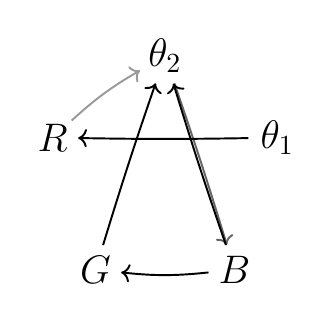
\begin{tikzpicture}
        \node[circle, inner sep=0.12em] (0) at (-1.427, 0.464) {\Large$R$};
        \node[circle, inner sep=0.12em] (1) at (-0.882, -1.214) {\Large$G$};
        \node[circle, inner sep=0.12em] (2) at (0.882, -1.214) {\Large$B$};
        \node[circle, inner sep=0.12em] (3) at (1.427, 0.464) {\Large$\theta_1$};
        \node[circle, inner sep=0.12em] (4) at (0.000, 1.500) {\Large$\theta_2$};
        \begin{scope}[]
            \draw[->, bend right=-6, line width = 0.7] (0) edge[color={rgb,1:red,0.6;green,0.6;blue,0.6}] (4);
            \draw[->, bend right=-1, line width = 0.7] (4) edge[color={rgb,1:red,0.4;green,0.4;blue,0.4}] (2);
            \draw[->, bend right=-1, line width = 0.7] (1) edge[color={rgb,1:red,0.0;green,0.0;blue,0.0}] (4);
            \draw[->, bend right=-6, line width = 0.7] (2) edge[color={rgb,1:red,0.0;green,0.0;blue,0.0}] (1);
            \draw[->, bend left=1, line width = 0.7] (2) edge[color={rgb,1:red,0.0;green,0.0;blue,0.0}] (4);
            \draw[->, bend left=1, line width = 0.7] (3) edge[color={rgb,1:red,0.0;green,0.0;blue,0.0}] (0);
        \end{scope}
    \end{tikzpicture}
\end{document}